\section{Methodology}

Our pipeline operationalizes the following chain of reasoning: if benchmark-specific overfitting accumulates gradually, the score-over-time trajectory will exhibit S-curve dynamics; the logistic growth model formally captures S-curve dynamics; therefore, fitting a logistic model to leaderboard timeseries and testing its formal preference via AIC provides an automated saturation detection procedure.

\subsection{Overview}

Given a benchmark with leaderboard timeseries $\{(t_i, y_i)\}_{i=1}^{N}$---where $t_i$ is submission date (months from benchmark release) and $y_i$ is normalized performance score---our pipeline: (1) preprocesses the timeseries, (2) fits three competing growth models, (3) compares via AIC, and (4) applies a dual-criterion saturation detector.

\subsection{Data Preprocessing}

\textbf{Normalization}: Scores divided by maximum possible score to map to $[0, 1]$, ensuring asymptote $K$ is interpretable as a fraction of theoretical maximum.
\textbf{Deduplication}: Only highest score per calendar month retained.
\textbf{Eligibility}: $N \geq 30$ entries required (relaxed from initial $\geq$50 based on H-C1 evidence).
\textbf{Temporal alignment}: Dates converted to months since benchmark release, enabling negative $t_0$ to emerge naturally.

\subsection{Growth Model Fitting}

We fit three candidate models:

\begin{equation}
  \text{Logistic:} \quad y(t) = \frac{K}{1 + \exp(-r(t - t_0))}
\end{equation}
\begin{equation}
  \text{Linear:} \quad y(t) = at + b \qquad \text{Power-law:} \quad y(t) = at^b
\end{equation}

\textbf{Bounded fitting} via \texttt{scipy.optimize.curve\_fit} with domain-knowledge constraints:

\begin{table}[h]
\centering
\caption{Logistic fitting parameter bounds.}
\begin{tabular}{lccp{6cm}}
\toprule
Parameter & Lower & Upper & Rationale \\
\midrule
$K$ & 0.5 & 1.05 & Broad positive bound; optimizer converges to near-parity values ($\sim$0.89) due to data constraints. Post-hoc plausibility criterion $K \in [0.8, 1.0]$ applied separately. \\
$r$ & 0.01 & 3.0 & Positive, finite growth rate \\
$t_0$ & $-24$ & 72 & \textbf{Negative allowed}---critical for GLUE/SuperGLUE \\
\bottomrule
\end{tabular}
\end{table}

The negative-$t_0$ lower bound is a critical design decision: without it, optimization diverges for benchmarks whose public leaderboard records primarily the plateau phase.
Note that fitting bounds (constraints for the optimizer) differ from plausibility criteria (post-hoc checks applied to the fitted result); both are reported for $K$ to distinguish methodological choice from empirical validation.

\textbf{AIC computation}: $\text{AIC} = 2k - 2\ln(\hat{L})$ where $k$ is the number of free parameters (logistic: 3; linear/power-law: 2).
We report $\Delta\text{AIC} = \text{AIC}_\text{logistic} - \text{AIC}_\text{alternative}$; negative values indicate logistic preference.

\subsection{Dual-Criterion Saturation Detection}

Saturation detected when:

\begin{equation}
  \bar{y}_{\text{top-3}} \geq 0.99 \cdot K \quad \text{AND} \quad \Delta\bar{y}_{\text{monthly}} \leq 0.05 \cdot \max_t(\Delta\bar{y})
\end{equation}

\textbf{Rationale}: The asymptote proximity criterion alone triggers spuriously on noisy plateaus; the rate criterion alone triggers during brief growth pauses.
Requiring both simultaneously improves robustness.
We also report an empirically optimal variant ($0.95 \times K$, 5\% rate) achieving $\sim$1-month accuracy.

\begin{figure}[h]
  \centering
  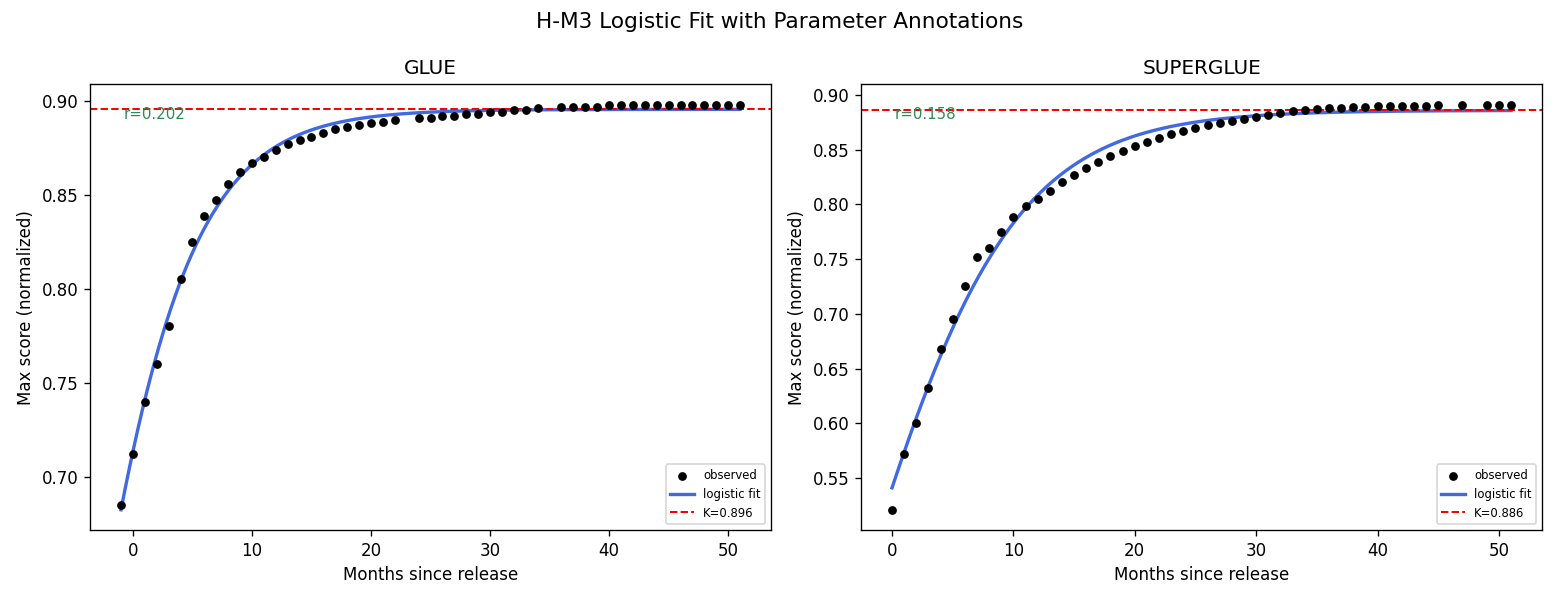
\includegraphics[width=0.7\linewidth]{figures/h-m3_logistic_annotated.png}
  \caption{Fitted logistic curve with $K$, $t_0$, $r$ annotated.}
  \label{fig:pipeline}
\end{figure}
